
\chapter[Numerical Methods for the System of Equations
  of...]{Numerical Methods for the System of Equations of 
  Hydrodynamics-Eulerian Coordinates}\label{chap10}   

\section{Introduction}\label{chap10:sec10.1}

In the\pageoriginale slab symmetric, one dimensional case, the
Eulerian form the equations of hydrodynamics is  
\begin{gather*}
\frac{\partial \rho}{\partial t} + \frac{\partial }{\partial x} (\rho
u) = 0 \tag{10.1}\label{eq10.1}\\ 
\frac{\partial (\rho u)}{\partial t} + \frac{\partial}{\partial x}
(\rho u^2 +  p + q) = 0 \tag{10.2}\label{eq10.2}\\ 
\frac{\partial}{\partial t} (\rho \epsilon) + \frac{\partial}{\partial
  x} (\rho u \epsilon)   + (p+q) \frac{\partial u}{\partial x} =0
\tag{10.3}\label{eq10.3} 
\end{gather*}
assuming $\mu$, $k$ and $g$ to be zero. Here $q$ is the pseudo-viscous term given by
\begin{equation*}
q = 2 \rho \Delta x^2 \max \left(0, - \frac{\partial u}{\partial x}\right)
\frac{\partial u}{\partial x}, \tag{10.4}\label{eq10.4} 
\end{equation*}
for a mesh of step $\Delta x$. Note that the equation (\ref{eq10.3}) can be written in terms of the total energy $E$ as 
\begin{equation*}
\frac{\partial}{\partial t} (\rho E) + \frac{\partial}{\partial x}
(\rho uE) + \frac{\partial}{\partial x} ((p+q) u) = 0
\tag*{$(10.3')$}\label{eq10.3'}  
\end{equation*}

The only interesting problem in the 1-dimensional Eulerian case is
that of a moving boundary (i.e. due to a piston or free surface
etc.). Unlike the Lagrangian system where, due to the same particles
lying on the free surface, the boundary is fixed, in the Eulerian case
the boundary moves with time. We will discuss this presently. To start
with we see how we can discretize the equation (\ref{eq10.1}) to
(\ref{eq10.3}) at an interior node of the mesh. One could use
characteristic, methods or the 2-step Lax-Wendroff scheme. We study
here the problems connected with the use of the leap-frog scheme. 

\section{Discretization at interior nodes}\label{chap10:sec10.2}

Assuming a uniform mesh with steps $\Delta x$ and $\Delta t$, we
compute as usual the quantities $p, \rho$ and $\epsilon$ at the
points\pageoriginale $(i+ \frac{1}{2}, n)$. We try to compute the
quantity $\rho u$ at $(i, n + \frac{1}{2})$ so that we can discretize
the equation (\ref{eq10.1}) by 
\begin{equation*}
\frac{\rho^{n+1}_{i+\frac{1}{2}} - \rho^n_{i+\frac{1}{2}}}{\Delta t} +
\frac{1}{\Delta x} \left[ (\rho u)^{n+\frac{1}{2}}_{i+1} - (\rho
  u)^{n+\frac{1}{2}}_i \right] =0 
\tag{10.5}\label{eq10.5}
\end{equation*}

Now we set $\bar{p} = p + q$. Then the equation (\ref{eq10.3}) can be discretized by
\begin{align*}
\frac{(\rho\epsilon)^{n+1}_{i+\frac{1}{2}} - (\rho
  \epsilon)^n_{i+\frac{1}{2}}}{\Delta t} & + \frac{1}{2}
\left(\bar{p}^{n+1}_{i+\frac{1}{2}} + \bar{p}^n_{i+\frac{1}{2}}\right)
\left(\frac{u^{n+\frac{1}{2}}_{i+1} - u^{n+\frac{1}{2}}_{i}}{\Delta x}\right)
+\\ 
& + \frac{1}{\Delta x} \left[ u^{n+\frac{1}{2}}_{i+1} (\rho \epsilon)^*_{i+1} - u^{n+\frac{1}{2}}_i (\rho \epsilon)^*_i\right] = 0,\tag{10.6}\label{eq10.6}
\end{align*}
where we set 
\begin{equation*}
(\rho \epsilon)^*_i = 
\begin{cases}
(\rho \epsilon)^n_{i+\frac{1}{2}}, \text{ if } u < 0\\
(\rho \epsilon)^n_{i-\frac{1}{2}}, \text{ if } u > 0. 
\end{cases}\tag{10.7}\label{eq10.7}
\end{equation*}

This is a 1-sided scheme and hence only of first order. However it is not as dissipative as Lax's scheme.

Notice however that due to the second term in (\ref{eq10.6}) one needs $u^{n+\frac{1}{2}}_i$ as well. This means that we need $\rho^{n+\frac{1}{2}}_i$ also (since we know $(\rho u)^{n+\frac{1}{2}}_i$). Thus effectively this method demands computation of $\rho$ not only at the points $(i+\frac{1}{2}, n)$ but also at the points $(i, n+ \frac{1}{2})$.

We now discretise equation (\ref{eq10.2}). We write
\begin{equation*}
\frac{(\rho u)^{n+\frac{1}{2}}_i - (\rho u)^{n-\frac{1}{2}}_i}{\Delta t} + \frac{1}{\Delta x} (\rho^n_{i+\frac{1}{2}} (u^*_{i+\frac{1}{2}})^2 - \rho^n_{i-\frac{1}{2}} (u^*_{i-\frac{1}{2}})^2) + \frac{\bar{p}^n_{i+\frac{1}{2}} - \bar{p}^n_{i-\frac{1}{2}}}{\Delta x}  = 0,
\tag{10.8}\label{eq10.8}
\end{equation*}
where
\begin{equation*}
u^*_{i+\frac{1}{2}} = 
\begin{cases}
u^{n-\frac{1}{2}}_{i+1}, \text{ if } u < 0\\
u^{n-\frac{1}{2}}_i , \text{ if } u > 0,
\end{cases}
\tag{10.9}\label{eq10.9}
\end{equation*}
is again a one-sided approximation.

We also\pageoriginale have 
\begin{equation*}
q^n_{i+\frac{1}{2}} = f(\rho^n_{i+\frac{1}{2}} (u^{n-\frac{1}{2}}_{i+1} - u^{n-\frac{1}{2}}_i)). 
\tag{10.10}\label{eq10.10}
\end{equation*}

As already remarked, the major problem is the additional computation of the values $\rho^{n+\frac{1}{2}}_i$. Of course, one has the immediate (but rather crude) approximation
\begin{equation*}
\rho^{n+\frac{1}{2}}_i = \frac{1}{2} (\rho^n_{i-\frac{1}{2}} + \rho^n_{i+\frac{1}{2}}). 
\tag{10.11}\label{eq10.11}
\end{equation*}

One could use a more sophisticated formula by applying Lax'\break scheme to
the equation of conservation of mass (i.e. (\ref{eq10.1})) to define
$\rho^{n+\frac{1}{2}}_i$. Thus we  
\begin{equation*}
\rho^{n+\frac{1}{2}}_i = \frac{1}{2} (\rho^n_{i+\frac{1}{2}} + \rho^n_{i-\frac{1}{2}}) - \frac{\Delta t}{2 \Delta x} (\rho^n_{i+\frac{1}{2}} u^n_{i+\frac{1}{2}} - \rho^n_{i-\frac{1}{2}} u^n_{i-\frac{1}{2}}). \tag{10.12}\label{eq10.12}
\end{equation*}
But then, we are faced with the need of computing $u^n_{i+\frac{1}{2}}$ as well. Thus we end up by computing both $u$ and $\rho$ at all nodes!

Noh \cite{key29} computed $\rho^{n+\frac{1}{2}}_i$ from $\rho^{n-\frac{1}{2}}_i$ and $\rho^{n-\frac{1}{2}}_{i+1}$ or $\rho^{n-\frac{1}{2}}_i$ and $\rho^{n-\frac{1}{2}}_{i-1}$ (according as $u<0$ or $>0$) using the one-sided scheme. The only draw back here is that $\rho^{n}_{i + \frac{1}{2}}$ is computed on the nodes $(i+\frac{1}{2}, n)$ and $\rho^{n+\frac{1}{2}}_i$ on the nodes $(i, n + \frac{1}{2})$ and these two grids are unconnected. On each grid one could get a good solution. But unless the mesh is very fine, when we put these values together the resulting function is not a good approximation of $\rho$.

However, all these methods give fairly satisfactory results.

\section{Treatment of boundary nodes}\label{chap10:sec10.3}
We will illustrate the discretization of the equation of conservation of mass ((\ref{eq10.1})) in case of a moving boundary. One can do the same for the other equations as well. It can be seen that the schemes in this case are fairly complicated.

To start\pageoriginale with, let us assume that the moving node at
$(n+1)\Delta t$ falls within the same grid-intervals as that at
$n\Delta t$ (See Fig. \ref{c10:fig10.1}). 

\begin{figure}[H]
\centering
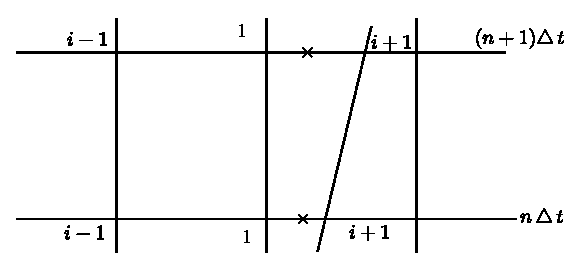
\includegraphics{figures/fig52-10.1.eps}
\caption{}\label{c10:fig10.1}
\end{figure}

One then has to compute $\rho$ at the mid-point of $(i, i +1)$ in the last interval. To discretise (\ref{eq10.1}) we imitate the following procedure for the continuous case:

Integrate $\rho$ between $x_i$ and $x_{i+1}(t)$ and differentiate w.r.t. $t$. Thus 
$$
\frac{d}{dt} \int\limits^{x_{i+1} (t)}_{x_i} \rho dx = \int\limits^{x_{i+1} (t)}_{x_i} \frac{\partial \rho}{\partial t} dx + \rho_{i+1} \frac{dx_{i+1} (t)}{dt} - \rho_i \frac{dx_i}{dt}. 
$$
Since $x_i$ is fixed and $S_{i+1}$ moves with velocity $u_{i+1}$, we get, on using equation (\ref{eq10.1}),
\begin{align*}
\frac{d}{dt} \int\limits^{x_{i+1}}_{x_i}\rho dx & = \rho_{i+1} u_{i+1} - \int\limits^{x_{i+1}}_{x_i} \frac{\partial}{\partial x} (\rho u) dx\\
& = \rho_{i+1} u_{i+1} - \rho_{i+1} u_{i+1} + \rho_{i} u_i = \rho_i u_i.
\end{align*}

We use this to discretise (\ref{eq10.1}). We write (at the boundary)
\begin{equation*}
\frac{1}{\Delta t} ((x^{n+1}_{i+1} - x_i) \rho^{n+1}_{i-\frac{1}{2}} - (x^n_{i+1} - x_i) \rho^n_{i+\frac{1}{2}}) = u_i \rho^*_i\tag{10.13}\label{eq10.13}
\end{equation*}
where\pageoriginale 
\begin{equation*}
\rho^*_i = 
\begin{cases}
\rho^n_{i+\frac{1}{2}}, \text{ if } u < 0\\
\rho^n_{i-\frac{1}{2}}, \text{ if } u > 0. 
\end{cases}
\tag{10.14}\label{eq10.14}
\end{equation*}

Let us now consider the case where the moving node is not in the same
grid interval at times $n\Delta t$ and $(n+1)\Delta t$. Again, this
splits into two cases one where the boundary has a forward slope and
thus there are more nodes at $(n+1)\Delta t$ than at $n\Delta t$
(Cf. Fig. \ref{c10:fig10.2} (a)) and the other where the boundary has a backward
slope and there are less points at $(n+1)\Delta t $ than at $n\Delta
t$ (Cf. Fig. \ref{c10:fig10.2} (b)) 

\begin{figure}[H]
\centering
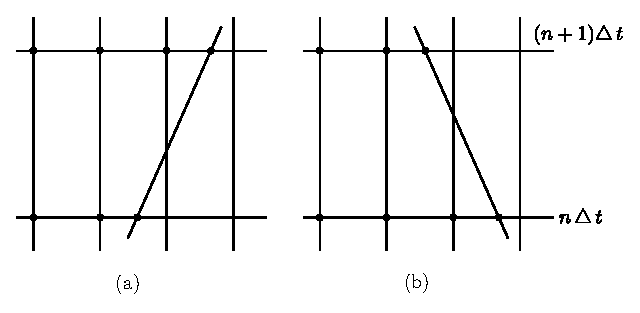
\includegraphics{figures/fig52-10.2.eps}
\caption{}\label{c10:fig10.2}
\end{figure}

We observe that as a result of these, the final mesh length may be too
small and for stability  reasons, this is not a satisfactory state of
affairs. Hence we choose our nodes such that the final mesh length
satisfies the condition 
\begin{equation*}
\frac{1}{2} \Delta x \leq (x_{I+1} - x_I) \leq \frac{3}{2} \Delta x.
\tag{10.15}\label{eq10.15}
\end{equation*}

Let us consider the case of Fig. \ref{c10:fig10.2} (a) where we have
more nodes at 
$(n+1)\Delta t$. We base our discussion on Fig. \ref{c10:fig10.3}. 

\begin{figure}[H]
\centering
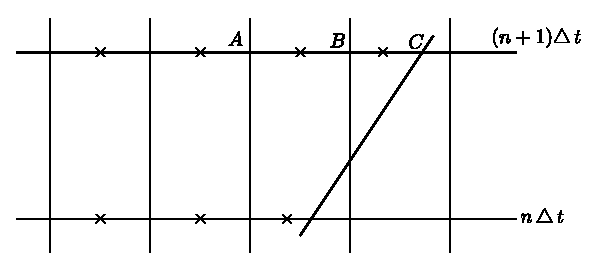
\includegraphics{figures/fig52-10.3.eps}
\caption{}\label{c10:fig10.3}
\end{figure}\pageoriginale

In order to discretise equation (\ref{eq10.1}) one must compute $\rho$ at the mid-points of the mesh lengths. One can do this for the interior points as before. Now one can ignore the node $B$ and treat AC as the last interval and using previous methods one can compute $\rho$ at the mid-point of AC. Let us call this $\rho^{\rm old}_{i+\frac{1}{2}}$. However, the length $x_C - x_A > \dfrac{3}{2} \Delta x $ and so one must split this as AB and BC and compute $\rho$ at the mid-points of these two intervals. If we call these values $\rho^{\rm new}_{i+\frac{1}{2}}$ and $\rho^{\rm new}_{i+3/2}$ respectively, we write
\begin{equation*}
\rho^{\rm old}_{i+\frac{1}{2}} (x_C - x_A) = \rho^{\rm new}_{i+\frac{1}{2}} (x_B- x_A) + \rho^{\rm new}_{i+3/2} (x_C - x_B). \tag{10.16}\label{eq10.16}
\end{equation*}

This together with another equation will help us to compute $\rho^{\rm
  new}_{i+\frac{1}{2}}$ and $\rho^{\rm new}_{i+3/2}$. For instance,
one can take $\rho^{\rm new}_{i+\frac{1}{2}}$ to be linearly
interpolated between $\rho^{\rm old}_{i-\frac{1}{2}} (=\rho^{\rm
  new}_{i-\frac{1}{2}})$ and $\rho^{\rm old}_{i+\frac{1}{2}}$. 

In the other case (Cf. Fig. \ref{c10:fig10.4}) we have $x_C - x_B <
\frac{1}{2} \Delta x$.  

\begin{figure}[H]
\centering
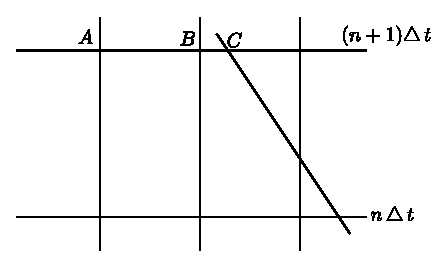
\includegraphics{figures/fig52-10.4.eps}
\caption{}\label{c10:fig10.4}
\end{figure}\pageoriginale

Here one can treat BC as a separate mesh length and thus we have equal number of nodes at $n$ and at $(n+1)$. Hence we can compute $\rho$ at the midpoints of AB and BC. However as $x_C-x_B < \frac{1}{2} \Delta x$, one must take AC as a whole interval. It $\rho^{\rm new}_{i+\frac{1}{2}}$ is the value of $\rho$ at the mid-point of AC, and $\rho^{\rm old}_{i+\frac{1}{2}}$ and $\rho^{\rm old}_{i+3/2}$ those at the mid-points of AB and BC, we write 
\begin{equation*}
\rho^{\rm new}_{i+\frac{1}{2}} (x_C - x_A) = \rho^{\rm old}_{i+\frac{1}{2}} (x_B - x_A) + \rho^{\rm old}_{i+3/2} (x_C - x_B)\tag{10.17}\label{eq10.17}
\end{equation*}
and we immediately get $\rho^{\rm new}_{i+\frac{1}{2}}$. 

Note that (\ref{eq10.16}) and (\ref{eq10.17}) merely approximate the fact that the mass contained in AC is the same as the total mass contained in AB and BC.

The problem of a moving boundary is complicated essentially because (i) the mesh is not longer uniform and (iii) the number of nodes involved in the computation varies as time proceeds. Hence if we are able to choose a coordinate system, i.e. rewrite the equation in terms of new variables, so that one can choose the nodes to move with the boundary, the situation  will improve. We discuss this possibility in the next subsection.

\section{The ale-method\protect
  \footnotemark[1]{}}\label{chap10:sec10.4}
\footnotetext[1]{Arbitrarily Lagrangian-Eulerian}

In this\pageoriginale method, we rewrite the equation in terms of a
new type of coordinates which is neither Lagrangian nor Eulerian. The
technique is comparatively new and has not yet been widely used.  

Let us assume that for each $t$ we have a homeomorphism $\varphi_t :
\mathbb{R} \to \mathbb{R}$ with the following properties: the mapping
$a \mapsto x(a,t) (=\varphi_t(a))$ (where $x = \varphi_\circ(a)$ at
time 0) is such that the Jacobian 
\begin{equation*} 
J = \frac{\partial x}{\partial a}\tag{10.19}\label{eq10.19}
\end{equation*}
is defined and is non-zero. We denote the derivative of $x$ w.r.t. $t$, when $a$ is fixed, by
\begin{equation*}
v= \frac{Dx}{Dt}.\tag{10.20}\label{eq10.20}
\end{equation*}

That is to say, a point initially at position a moves with velocity $v$ and its position at time $t$ is given by $x=x(a,t)$. The various `trajectories' do not cross one another and this is meaning of the condition that $J \neq 0$. Note that for the Lagrangian coordinate system we have $v = u$, the velocity of the fluid. In case of the Eulerian system $x$ never changes and hence $J=1$ and $v=0$. Thus this type of coordinate system contains both the Lagrangian and Eulerian systems as particular cases.

If one knows a function $(x,t) \mapsto \varphi(x,t)$ we define $\bar{\varphi} (a,t)$ by 
\begin{equation*}
\bar{\varphi} (a,t) = \varphi (x(a,t).t)\tag{10.21}\label{eq10.21}
\end{equation*}
and one has 
\begin{equation*}
\frac{D\bar{\varphi}}{Dt} = \frac{\partial \varphi}{Dt} + v \frac{\partial \varphi}{\partial x}, \tag{10.22}\label{eq10.22}
\end{equation*}
Here\pageoriginale $\dfrac{D\bar{\varphi}}{Dt}$ means the derivative
of $\bar{\varphi}$ with respect to $t$ when $a$ is kept fixed. We now
rewrite the equation (\ref{eq10.1}) in terms of this systems: c
\begin{align*}
\frac{D}{Dt} (\rho J) & = \rho \frac{DJ}{Dt} + J \frac{D\rho}{Dt}\\
& = \rho \frac{\partial v}{\partial a} + J (\frac{\partial
  \rho}{\partial t} + v \frac{\partial \rho}{\partial x})\\ 
& =  \rho \frac{\partial v}{\partial a} + J \left(v \frac{\partial
  \rho}{\partial x} - \frac{\partial}{\partial x} (\rho u)\right) \;
(\text{using (\ref{eq10.1})})\\ 
& = \rho \frac{\partial v}{\partial a} + v \frac{\partial
  \rho}{\partial a} - \frac{\partial}{\partial a} (\rho u) =
\frac{\partial}{\partial a} (\rho (v-u)). 
\end{align*}
Thus (\ref{eq10.1}) now takes the form 
\begin{equation*}
\frac{D}{Dt} (\rho J) + \frac{\partial}{\partial a} (\rho (u-v)) = 0.
\tag{10.23}\label{eq10.23}
\end{equation*}

By doing the same thing for the other two equations one has 
\begin{equation*}
\frac{D}{Dt} (\rho u J) + \frac{\partial}{\partial a} (\rho u (u-v) + p) = 0,
\tag{10.24}\label{eq10.24}
\end{equation*}
and
\begin{equation*}
\frac{D}{Dt} (\rho \epsilon J) + \frac{\partial}{\partial a} (\rho \xi (u-v)) + p \frac{\partial u}{\partial a} = 0. \tag{10.25}\label{eq10.25}
\end{equation*}

\begin{remark}\label{chap10:rem10.1}
In view of our comments made previously, the above equations contain the Lagrangian and Eulerian equations as particular cases.
\end{remark}

Let us now take a fixed $(a-t)$ grid. We define $x$ at the points $(i,n), u$ at the points $(i, n + \frac{1}{2})$, and $J$, $\rho$ at the points $(i+\frac{1}{2},n)$, thus we write the discrete equations
\begin{align*}
& x^{n+1}_i  - x^n_i = v^{n+\frac{1}{2}}_i \Delta t. 
\tag{10.26}\label{eq10.26}\\
& J^{n+1}_{i+\frac{1}{2}}  = \frac{x^{n+1}_{i+1} - x^{n+1}_i}{a_{i+1} - a_i}, 
\tag{10.27}\label{eq10.27}
\end{align*}
and 
\begin{align*}
&  \frac{1}{\Delta t} \left[\rho^{n+1}_{i+\frac{1}{2}} J^{n+1}_{i+\frac{1}{2}} - \rho^n_{i+ \frac{1}{2}} J^n_{i+\frac{1}{2}}  \right] +\\
&  \qquad + \frac{1}{(a_{i+1} - a_i)} \left[(u-v)^{n+\frac{1}{2}}_{i+1} \rho^*_{i+1} - (u-v)^{n+\frac{1}{2}}_i \rho^*_{i} \right] = 0 \tag{10.28}\label{eq10.28}
\end{align*}\pageoriginale
with, for example,
\begin{equation*}
\rho^*_{i+1} = 
\begin{cases}
\rho^n_{i+3/2}, \text{ if } u - v < 0\\
\rho^n_{i+\frac{1}{2}}, \text{ if } u - v > 0
\end{cases}\tag{10.29}\label{eq10.29}
\end{equation*}
if one uses a one-sided scheme. This discretizes the equation (\ref{eq10.23}). One can similarly discretise the other equations of hydrodynamics as well.

\begin{remark}\label{chap10:rem10.2}
The equations (\ref{eq10.27}) and (\ref{eq10.28}) give 
\begin{multline*}
\left[\rho^{n+1}_{i+\frac{1}{2}} (x^{n+1}_{i+1} - x^{n+1}_i) -
  \rho^n_{i+\frac{1}{2}} (x^n_{i+1} - x^n_i) \right]\\ 
= \Delta t \left[
  -(u-v)^{n+\frac{1}{2}}_{i+1} \rho^*_{i+1} +(u-v)^{n+\frac{1}{2}}_i
  \rho^*_{i}\right].  
\end{multline*}
This merely states that if $M^{n+1}_{i+\frac{1}{2}}$ is the mass at time $n+1$ between the nodes $i$ and $i+1$, then 
\begin{align*}
& M^{n+1}_{i+\frac{1}{2}} - M^n_{i+\frac{1}{2}} = \\
& \quad = [\text{Inflow into the cell $(i, i+1)$}] - [\text{Outflow from the cell $(i,i+1)$}]. 
\end{align*}
The use of the one-sided scheme to define $\rho^*_i$ then says, that one ought to define the density at the boundary of the cell to be the one inside the cell from which the fluid is flowing through that boundary. This is why the above equation is some times called the {\em Donor-cell equation}.
\end{remark}

At each time $n+1$, we have to define $v^{n+\frac{1}{2}}_i$ or, equivalently $x^{n+1}_i$. One can, for example, define $x$ such that the mesh is always uniform. To avoid the free surface crossing the grid one can take $v$ on the surface to be the velocity of the surface itself. This is the merit of this method.

For most of the $1$-dimensional problems, the Lagrangian coordinate system\pageoriginale is good enough (i.e. the preceding method with $v=u$), because there is no problem of distortion of the mesh. This is no longer true in the 2-dimensional problems where the generalization of the ALE method may come in very useful when dealing with boundaries moving w.r.t. a frame fixed in the laboratory.

As for comparing the Lagrangian and Eulerian systems, it is clear that the Lagrangian method is preferable. In pseduo-viscosity methods Eulerian methods involve fine meshes about a shock. In case of Lagrangian systems the mesh will be automatically fine near a compression or shock without increasing the number of nodes. Thus it is more feasible from the point of view of computers.

This brings us to a close of the discussion of one dimensional time
dependent equations. In the next section we will take up
two - dimensional problems. 
